\documentclass[letterpaper, 12pt]{math}

\usepackage{amsmath}
\usepackage{pgfplots}
\pgfplotsset{compat=1.8}
\usetikzlibrary{arrows}

\title{Multivariable and Vector Calculus}
\author{Alvin Lin}
\date{August 2017 - December 2017}

\begin{document}

\maketitle

\section*{Cartesian Coordinates}
We take a standard x-y plane and put another axis perpendicular to it called
the z-plane and plot points as \( (x, y, z) \). This is known as the Cartesian
coordinate system.
\begin{center}
  \begin{tikzpicture}[x=0.2cm,y=0.2cm,z=0.2cm]
    % The axes
    \draw[->] (xyz cs:x=-13.5) -- (xyz cs:x=13.5) node[above] {$x$};
    \draw[->] (xyz cs:y=-13.5) -- (xyz cs:y=13.5) node[right] {$z$};
    \draw[->] (xyz cs:z=-13.5) -- (xyz cs:z=13.5) node[above] {$y$};

    \node[fill,circle,inner sep=1.5pt,label={below:\( (x_{1},y_{1},z_{1}) \)}]
      at (-3,-4,2) {};
    \node[fill,circle,inner sep=1.5pt,label={above:\( (x_{2},y_{2},z_{2}) \)}]
      at (3,5) {};
  \end{tikzpicture}
\end{center}

\noindent Cartesian Distance:
\[ d((x_{1}, y_{1}, z_{1}), (x_{2}, y_{2}, z_{2})) = \sqrt{
  (x_{2}-x_{1})^{2}+(y_{2}-y_{1})^{2}+(z_{2}-z_{1})^{2}} \]
Sphere of radius \( r \), center \( (x_{\circ},y_{\circ},z_{\circ}) \):
\[ (x-x_{\circ})^{2}+(y-y_{\circ})^{2}+(z-z_{\circ})^{2} = r^{2} \]

\subsection*{Example}
Give the largest sphere with center at \( (2,7,5) \) which fits within the I
octant \( (x>0,y>0,z>0) \).
\[ (x-2)^{2}+(y-7)^{2}+(z-5)^{2} = 2^{2} \]

\subsection*{Example}
\[ x^{2}+y^{2}+z^{2}-4x+2y-6z = 1 \]
What is the center and radius of such a circle?
\begin{align*}
  x^{2}-4x+y^{2}+2y+z^{2}-6z &= 1 \\
  x^{2}-4x+y^{2}+2y+z^{2}-6z &= 1 \\
  [(x-2^{2})-4]+[(y+1)^{2}-1]+[(z-3)^{2}-9] &= 1+4+1+9 \\
  (x-2)^{2}+(y+1)^{2}+(z-3)^{2} &= 15 \\
\end{align*}

\subsection*{Example}
Are the points \( P_{1}(1,2,3) \), \( P_{2}(2,3,4) \), \( P_{3}(0,2,6) \)
colinear?
\[ dist(P_{1},P_{2}) = \sqrt{3} \]
\[ dist(P_{2},P_{3}) = 3 \]
\[ dist(P_{1},P_{3}) = \sqrt{10} \]
Two of the distances should sum up to the third. This is not true for any of
these, thus the lines are not colinear.

\subsection*{Graphing in 3D}
Graph \( y = x^{2} \):
\begin{center}
  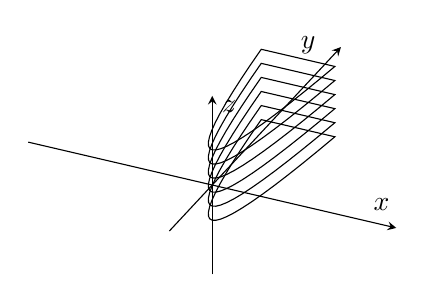
\begin{tikzpicture}
    \begin{axis}[
        axis equal,
        axis lines = center,
        xlabel = {$x$},
        ylabel = {$y$},
        zlabel = {$z$},
        enlargelimits = 0.5,
        ticks=none
    ]
      \addplot3[
          variable = \x,
          variable y = \y,
      ]({x}, {x^2}, {1});
      \addplot3[
          variable = \x,
          variable y = \y,
      ]({x}, {x^2}, {-1});
      \addplot3[
          variable = \x,
          variable y = \y,
      ]({x}, {x^2}, {3});
      \addplot3[
          variable = \x,
          variable y = \y,
      ]({x}, {x^2}, {-3});
      \addplot3[
          variable = \x,
          variable y = \y,
      ]({x}, {x^2}, {5});
      \addplot3[
          variable = \x,
          variable y = \y,
      ]({x}, {x^2}, {-5});
    \end{axis}
  \end{tikzpicture}
\end{center}
This graph extends up and down the z axis infinitely and form a surface.

\section*{Vectors}
\[ A(a_{1},a_{2},a_{3}) \]
\[ B(b_{1},b_{2},b_{3}) \]
\[ \vec{AB} = \langle b_{1}-a_{1},b_{2}-a_{2},b_{3}-a_{3}\rangle \]

\subsection*{Vector Operations}
\[ \vec{a}+\vec{b} = \langle a_{1}+b_{1},a_{2}+b_{2},a_{3}+b_{3}\rangle \]
\[ \lambda\vec{a} = \langle\lambda a_{1},\lambda a_{2},\lambda a_{3}\rangle \]
\[ |\vec{a}| = \sqrt{a_{1}^{2}+a_{2}^{2}+a_{3}^{2}} \]
\[ |\lambda\vec{a}| = |\lambda||\vec{a}| \]
\[ \lambda(\vec{a}+\vec{b}) = \lambda\vec{a}+\lambda\vec{b} \]
\[ \vec{a} = \langle a_{1},a_{2},a_{3}\rangle =
  |\vec{a}|\langle\frac{a_{1}}{|\vec{a}|}\frac{a_{2}}{|\vec{a}|}
  \frac{a_{3}}{|\vec{a}|}\rangle =
  |\vec{a}|\langle\cos(\alpha),\cos(\beta),\cos(\gamma)\rangle \]

\subsection*{Example}
Draw \( 2\vec{a}-\frac{1}{3}\vec{b} \):
\begin{center}
  \begin{tikzpicture}[scale=0.8]
    \node (O) at (0,0) {O};
    \node (A) at (2,2) {\( \vec{a} \)};
    \node (2A) at (4,4) {\( 2\vec{a} \)};
    \node (B) at (6,-3) {\( \vec{b} \)};
    \node (13B) at (-2,1) {\( \frac{1}{3}B \)};
    \node (SUM) at (2,5) {\( 2\vec{a}-\frac{1}{3}\vec{b} \)};
    \draw[->] (O) edge (B);
    \draw[->] (O) edge (A);
    \draw[->] (O) edge (2A);
    \draw[->] (O) edge (13B);
    \draw[->] (O) edge (SUM);
  \end{tikzpicture}
\end{center}

\subsection*{Example}
Given the vector of length 7 which makes an angle of \( 15^{\circ} \) with
\( \langle3,3\rangle \).
\[ \vec{a} = 7\langle\cos(30),\cos(60)\rangle =
  7\langle\frac{\sqrt{3}}{2},\frac{1}{2}\rangle =
  \langle\frac{7\sqrt{3}}{2},\frac{7}{2}\rangle \]
Alternate Solution:
\[ \vec{a} = 7\langle\cos(60),\cos(30)\rangle =
  7\langle\frac{1}{2},\frac{\sqrt{3}}{2}\rangle =
  \langle\frac{7}{2},\frac{7\sqrt{3}}{2}\rangle \]

\subsection*{Example}
A pilot steers a plane at 500mph towards N 30 E, while the wind blows at 200mph
from N 45 W. Find the true course and speed.
\begin{align*}
  \vec{t} &= \vec{pilot}+\vec{wind} \\
  &= 500\langle\cos(60),\cos(30)\rangle+200\langle\cos(45),-\cos(45)\rangle \\
  &= \langle250,250\sqrt{3}\rangle+\langle100\sqrt{2},-100\sqrt{2}\rangle \\
  &= \langle250+100\sqrt{2},250\sqrt{3}-100\sqrt{2}\rangle
\end{align*}

\begin{center}
  If you have any questions, comments, or concerns, please contact me at
  alvin@omgimanerd.tech
\end{center}

\end{document}
